% !TEX encoding = UTF-8 Unicode

\documentclass[twocolumn,10pt,a4j]{jsarticle}
\usepackage{kougai}

\title{積み上げ型教科の理解を促進させる
教育モデルの提案}
\author{1532009 阿部 希駿  指導教員 須田 宇宙 准教授}
\date{}

\begin{document}

\maketitle

\section{はじめに}

%背景
中学,高校で学習する科目の中で数学と英語は苦手になりやすいと言われている\cite{1}.この2科目の共通点として既に学習した知識を使うことを前提として授業を行う「積み上げ型教科」という点が挙げられる.積み上げ型教科では単元の内容が複雑になるほど必要な前提知識が多くなり,使用する単元がわかりにくくなる.そのためその単元の内容を理解をすることが難しくなることが問題点としてあげられる.

%問題点

そこで学習する単元を前提知識とする単元の概要をあらかじめ学習することで,個々の単元の理解を促進することができるという仮説を立てた.
本研究では,学生を対象にして実験を行い,この仮説を証明することを目的とする.


\section{実験の構想}

本研究では2018年後期に開講される情報数学応用の講義履修者を対象に9週目,10週目,11週目の講義にて対照実験を行う.
図\ref{fig:time}に示すように9週目と10週目に講義を行い,11週目に小テストを行う.

\begin{figure}[H]
\centering
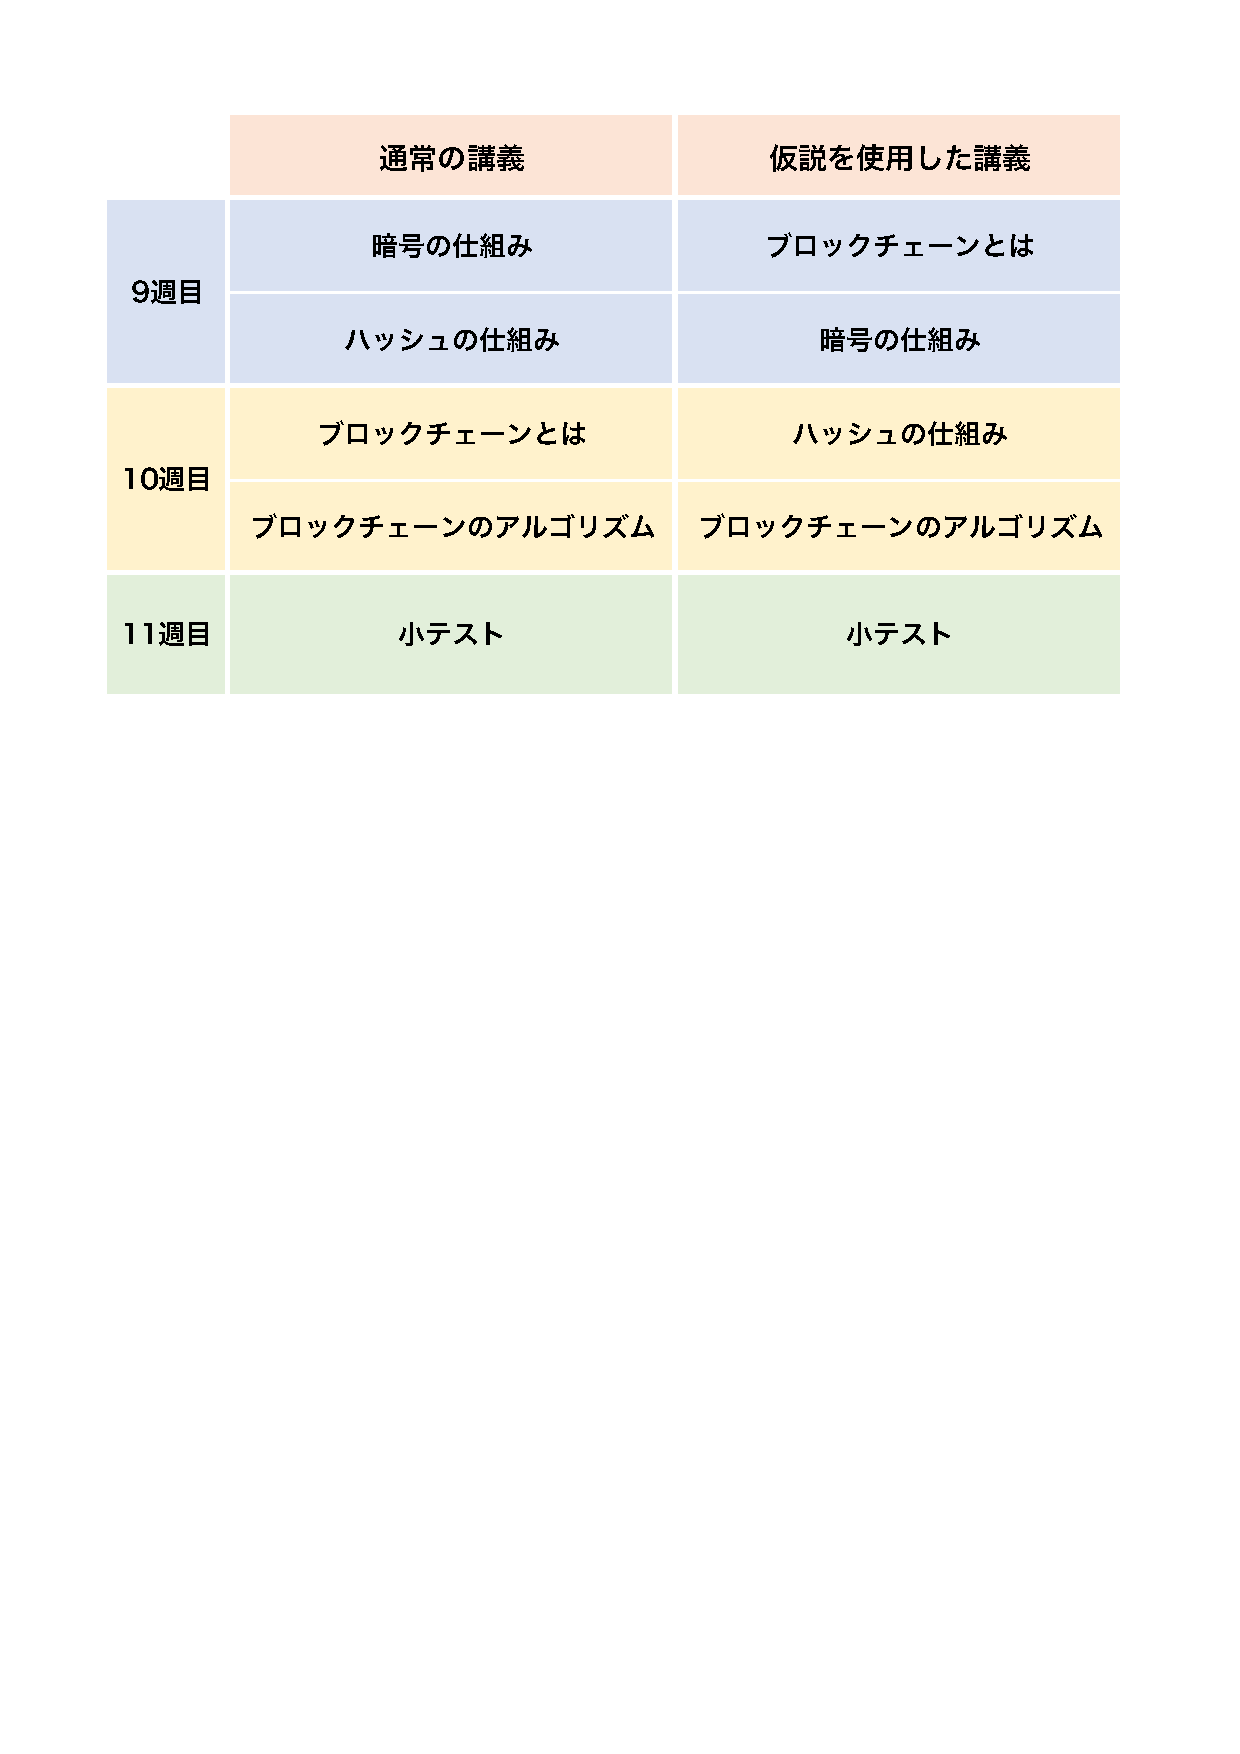
\includegraphics[mediaboxonly=/CropBox,width=9cm]{timeline.pdf}
\caption{実験で行う授業の流れ}
\label{fig:time}
\end{figure}
Bクラスでは通常の流れで講義を行い,Aクラスでは仮説を基に変更した流れで講義を行う.
仮説を基に変更した講義ではブロックチェーンの概要を学習した後に暗号とハッシュについて学習し,もう一度ブロックチェーンの学習に戻り詳細に学習する.


小テストでは以下の3項目の問題とアンケートを用意する.
\begin{enumerate}
\renewcommand {\labelenumi}{(\arabic{enumi})}
\item 暗号の仕組み
\item ハッシュと暗号の違い
\item ブロックチェーンの仕組み
\end{enumerate}

アンケートでは講義を受ける以前にブロックチェーンの仕組みについての知識の有無について尋ねた.
結果の分析は小テストの点数を「暗号・ハッシュ」「ブロックチェーン」の二項目について行う.
また2クラスの元の学力の影響を考え,中間試験と小テストの平均点を調べる.
そこで小テストの分析対象を中間試験の受験者かつブロックチェーンを講義前に学習していない学生とした.


\section{考察}

小テストの結果,2クラスの点数に差は見られなかった.図\ref{fig:total}では合計点の得点分布を示す.

\begin{figure}[H]
\centering
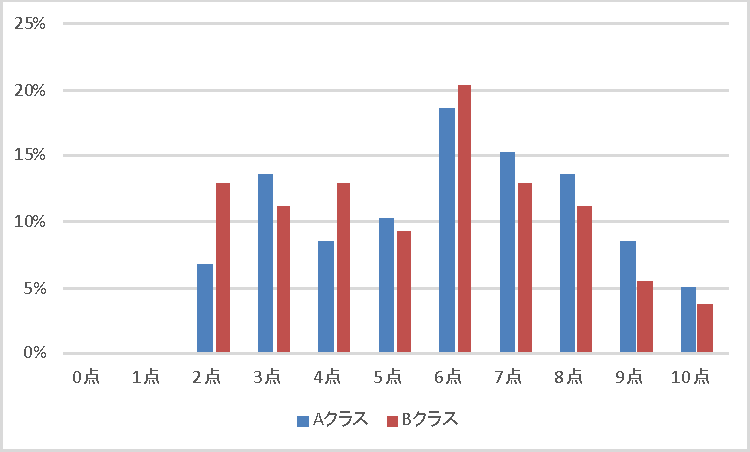
\includegraphics[width=8cm]{total.pdf}
\caption{小テストの合計点の得点分布}
\label{fig:total}
\end{figure}

仮説が証明できなかった原因を考察した.
\begin{itemize}
\item 仮説が間違えている
\item 小テストを行うまでに期間が空いた
\item 実験を行う教科が不適であった
\item 問題の難易度に差が見られた
\end{itemize}

「暗号・ハッシュ」と「ブロックチェーン」の平均点に大きく差が見られたことから,前半にブロックチェーンの概要を学習したクラスの得点が下がった可能性がある.また小テストを行う事前予告をした上で,期間を空けたために,テスト勉強を行った学生の人数の差が大きかった可能性があり,純粋な講義のみの理解度を測ることができなかった可能性を考えた.

\section{おわりに}
本研究では積み上げ型教科の理解度を上げる仮説を立て,実験を行なった.今回の実験では仮説が正しいと証明することができなかったが,実験の改善点が見つかったため,今後はさらなる実験を行い検証することが望まれる.

\begin{thebibliography}{99}
\bibitem{1}
ベネッセ教育情報サイト:“教科学習が不得意と感じている高校生が9割!そのほとんどが英語と数学に偏るのにはある理由が”, \url{https://www.benesse.jp/kyouiku/201603/20160329-3.html}, (参照 2018-8-14)
\end{thebibliography}

\end{document}